%-----------------------------------------------------------------------------
%
%               Template for sigplanconf LaTeX Class
%
% Name:         sigplanconf-template.tex
%
% Purpose:      A template for sigplanconf.cls, which is a LaTeX 2e class
%               file for SIGPLAN conference proceedings.
%
% Guide:        Refer to "Author's Guide to the ACM SIGPLAN Class,"
%               sigplanconf-guide.pdf
%
% Author:       Paul C. Anagnostopoulos
%               Windfall Software
%               978 371-2316
%               paul@windfall.com
%
% Created:      15 February 2005
%
%-----------------------------------------------------------------------------


\documentclass[numbers]{sigplanconf}

% The following \documentclass options may be useful:

% preprint      Remove this option only once the paper is in final form.
% 10pt          To set in 10-point type instead of 9-point.
% 11pt          To set in 11-point type instead of 9-point.
% numbers       To obtain numeric citation style instead of author/year.

\usepackage{amsmath, amssymb, float, caption,graphicx}
\usepackage[ruled,vlined]{algorithm2e}
\usepackage{color}
\usepackage[dvipsnames]{xcolor}


\newcommand{\cL}{{\cal L}}

\begin{document}

\special{papersize=8.5in,11in}
\setlength{\pdfpageheight}{\paperheight}
\setlength{\pdfpagewidth}{\paperwidth}

\conferenceinfo{CONF 'yy}{Month d--d, 20yy, City, ST, Country}
\copyrightyear{20yy}
\copyrightdata{978-1-nnnn-nnnn-n/yy/mm}
\copyrightdoi{nnnnnnn.nnnnnnn}
\allowdisplaybreaks

% Uncomment the publication rights you want to use.
%\publicationrights{transferred}
%\publicationrights{licensed}     % this is the default
%\publicationrights{author-pays}

\titlebanner{banner above paper title}        % These are ignored unless
\preprintfooter{short description of paper}   % 'preprint' option specified.

\title{GRAMPA: Generalized Rick And Morty ProgrAmming}
\subtitle{Contact: [email]@grinnell.edu}

\authorinfo{Reilly Grant}
           {Grinnell College}
           {[grantrei]}
\authorinfo{Tristan Knoth}
           {Grinnell College}
           {[knothtri17]}
\authorinfo{Chris Kottke}
           {Grinnell College}
           {[kottkech17]}

\maketitle

\begin{abstract}
Parallel computing is an important way to process over very large problems. However, developing parallel applications is extremely difficult. We develop Generalized Rick And Morty ProgrAmming (GRAMPA), an esoteric imperative programming language supporting a simple forking model in order to simulate parallelism and introduce students shared memory and other rudimentary parallel computing concepts. The language supports only a limited set of commands, and includes syntax is based on the popular cartoon Rick and Morty in order to present parallel computing concepts in a fun and accessible manner.
\end{abstract}

\section{Introduction}

As parallelism becomes the most important paradigm for large-scale information processing, developing parallel applications is becoming an increasingly important skill for any developer. Students who begin to think about splitting problems up between processors earlier in their computer science education will potentially see more success learning more sophisticated parallelism paradigms later on. To this end, the popular TV show Rick and Morty presents the perfect medium through which to introduce students to rudimentary parallelism concepts. We develop GRAMPA, a simple Turing Complete imperative language with syntax based on references to Rick and Morty that supports a simple model of forking across shared memory. In Rick and Morty, the main characters travel between dimensions. The show's clear conceptual connections to multithreading may help alleviate the pain of learning to parallelize simple algorithms. GRAMPA's syntax is intended to look something like written natural language.

\section{Prior Work}

GRAMPA relies on a number of existing technologies, particularly the Haskell Parsec library. Our parser is built in Haskell using Parsec, which allows users to combine parsers via monads.... Didn't really know what else to put in this section.

\section{Examples}
An example programming using two threads to find all prime numbers less than 1000 is in appendix A. One thread processes half the odd numbers (1, 5, 9, $\ldots$) and the other processes the other half of the odd numbers (3, 7, 11 $\ldots$). 

\section{Parsing GRAMPA}

Using Parsec, we can build a recursive descent parser for GRAMPA by combining parsers for different types of expressions and statements in our language. Given a grammar for our language, we can define parsers for each variable in the grammar and thus recursively parse the entire language.

\subsection*{Grammar}
The following Context-Free Grammar defines the GRAMPA syntax, and indicates the parsing hierarchy. The variable STRING refers to any string consisting only of chars, and INT refers to any integer.
\begin{align*}
	S &\rightarrow UNIV \\
	UNIV &\rightarrow \text{universe } STRING \; STMT \text{ destroy universe } \mid UNIV \; UNIV \\
	STMT &\rightarrow PORTAL \mid IF \mid DECL \mid PRINT \mid WHILE \mid STMT \; STMT \\
	EXPR &\rightarrow OP1 \\
	OP1 &\rightarrow AND \mid OR \mid OP2 \\
	OP2 &\rightarrow NUMEQ \mid NUMLT \mid NUMGT \mid OP3 \\
	OP3 &\rightarrow ADD \mid SUB \mid OP4 \\
	OP4 &\rightarrow MUL \mid DIV \mid MOD \mid TERM \\
	TERM &\rightarrow BASE \mid PARENA \mid PARENB \mid STRING \\
	BASE &\rightarrow INT \mid BOOL \\
	BOOL &\rightarrow \text{right} \mid \text{wrong} \\
	PORTAL &\rightarrow \text{lets grab our } STRING \text{ and portal out of here}\\
	IF &\rightarrow \text{if } OP1 \text{ then } STMT \text{ otherwise } STMT \text{ wubulubadubdub}\\
	DECL &\rightarrow STRING \text{ means } EXPR\\
	PRINT &\rightarrow \text{show me } STRING\\
	WHILE &\rightarrow \text{while } OP1 \text{ do this for grandpa } STMT \text{ thanks Summer}\\
	AND &\rightarrow OP2 \text{ and } OP1\\
	OR &\rightarrow OP2 \text{ or } OP1\\
	NUMEQ &\rightarrow OP3 \text{ is the same as } OP3 \\
	NUMLT &\rightarrow OP3 \text{ is less than } OP3\\
	NUMGT &\rightarrow OP3 \text{ is greater than } OP3\\
	ADD &\rightarrow OP4 \text{ plus } OP3\\
	SUB &\rightarrow OP4 \text{ minus } OP3\\
	MUL &\rightarrow TERM \text{ times } OP4\\
	DIV &\rightarrow TERM \text{ divided by } OP4\\
	MOD &\rightarrow TERM \text{ mod } OP4\\
	PARENA &\rightarrow \text{you gotta } OP3 \text{ Morty}\\
	PARENB &\rightarrow \text{you gotta } OP1 \text{ Morty}\\
\end{align*}

Given the context-free grammar above, we define parsers for each of the individual substitution rules. For example, to parse a multiplication, we look for a $TERM$ on the left side of the expression, a "times" to indicate that we are multiplying two expressions, and an $OP4$ on the right hand side of the expression. In Haskell, this is implemented as follows:

\begin{algorithm}
	\texttt{whitespace} \\
	\texttt{e1} $\leftarrow$ \texttt{termParser}\\
	\texttt{whitespace} \\
	\texttt{string} "times" \\
	\texttt{whitespace} \\
	\texttt{e2} $\leftarrow$ \texttt{op4Parser} \\
	\texttt{whitespace} \\
	\texttt{return} \$ EBin Mul e1 e2  \\
	\caption{Multiplication Parser}
\end{algorithm}

The sequence of instructions above is wrapped in a "do" block to create a parser for multiplication. \texttt{whitespace} is a parser designed to consume all whitespace. As such, our language is completely whitespace insensitive as long as one separates commands by any amount of whitespace. \texttt{string} is a parser built into Parsec, which parses a specific string. In this way, we combine parsers for different types of expressions and recursively parse the entire document. 

Parsec also gives the user the option to "try" a parser. If one uses "try" when calling a specific parser, the parser will only consume input if it successfully parses the entire expression. Thus, if it encounters an error it will attempt again to parse the exact same string for a different type of expression. This feature allows us to combine parsers for different types of expressions quite easily. For example, we parse statements, which have a number of forms, in the following way:

\texttt{stmt = try sPortal <|> try sIf <|> try sDec <|> try sPrint <|> try sWhile}

Thus, if the parser does not find an "if" statement, it can move on to look for a variable declaration or a print statement, for example. "Trying" different parsers in this way allows us to combine parsers like the multiplication parser described above and recursively parse the entire context-free grammar. 

As a final note, one should observe that our order of operations is implicitly embedded in the grammar, and therefore the parser. The relevant portion of the grammar begins with the $EXPR \rightarrow OP1$ substitution. Here, we parse operations in ascending precedence. We parse the terminals and parenthesized expressions last in order to ensure that they are leafs in the parse tree and are therefore evaluated first. 

Our parsing methodology leads to a few idiosyncrasies in GRAMPA. For example, if statements must execute statements in both the true and false cases. In other languages, programmers can often simply omit the "else" case if it is unnecessary. However, when writing GRAMPA code, if one does not want anything to execute in the "else" case, one must include a dummy instruction, such as assigning a never-used variable.

\subsection{Left Associativity}
Parsing a file using the process described above results in a right-associative parse tree. 
This means that the expression $1 + 2 + 3$ is parsed as $1 + (2 + 3)$ rather than $(1 + 2) + 3$,
which is what one would expect. In many cases this difference is nontrivial. For example, we need to
ensure that $16 / 4 / 2$ evaluates to $(16 / 4) / 2 = 2$ rather than $16 / (4 / 2) = 8$. To rectify this
problem, we transform the abstract syntax tree(AST) generated by our parser to reorder operations and 
guarantee left-associativity. Initially, we attempted to generate the AST to be left associative,
but found that difficulty learning and using Parsec, made this task more difficult than just changing that AST 
after parsing. The algorithim we used was based on the following observation, consider  1 -2 -3 -4, we see that
with right associativity, that this is parsed as  (1 -(2 - 3), and if it is parsed with left associativity, that it is parsed
((1-2) -3). As a tree, this is represented as 

$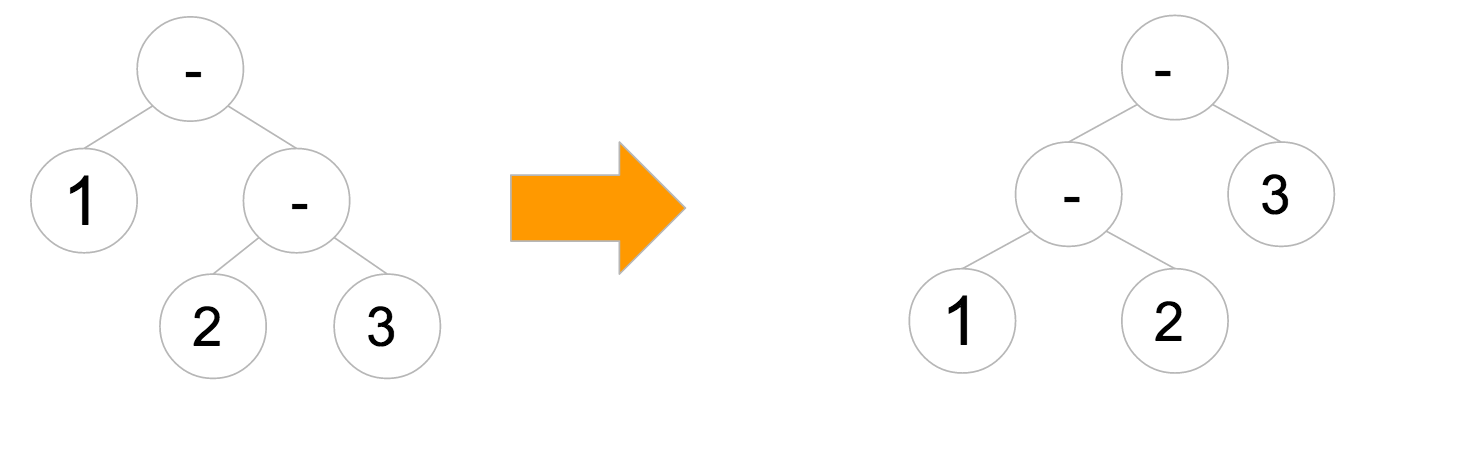
\includegraphics[width=\linewidth]{ASTtransformex1}$

We see that this can be represented generally as a change of   (a op1 (b op2 c)) to ((a op1 b) op2 c). 
This change in a tree is represented as

$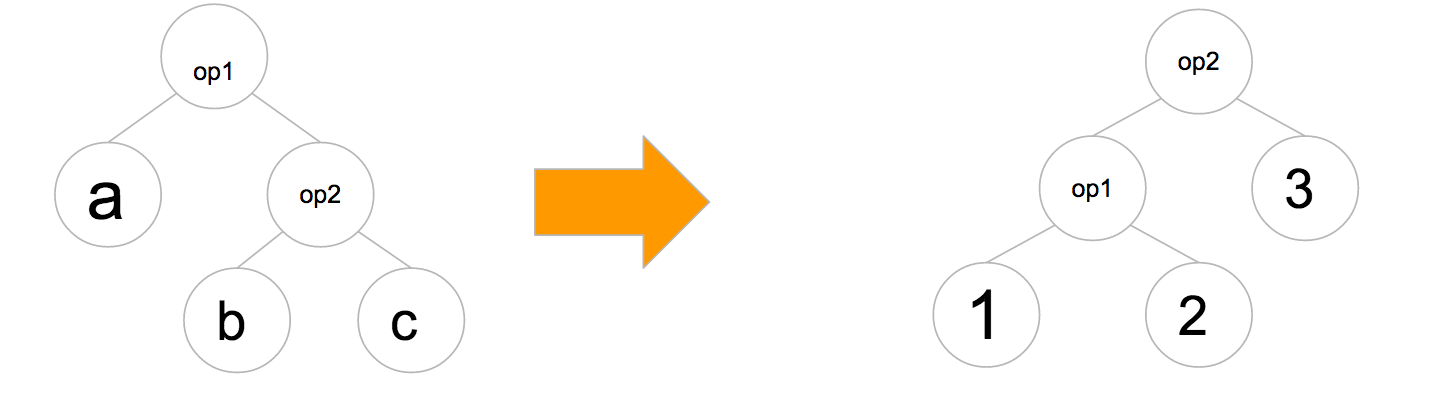
\includegraphics[width=\linewidth]{ASTtransformex2}$

We also see that if we repeatedly apply this transformation until the right child of the top node is either parens, 
or a literal, and then recurses on all children, that we have an algorithim that changes a right-associative parse tree
into a left-associative parse tree. 

One additional note is that to preserve order of operations, addition and subtraction treat a right child 
which is multiplication or division node as a literal, in that the structure tree remains the same, 
except for recursing on the right child. The function we used to do this transformation is used after all parsing 
is done, and maps over all universes, and all statements in all universes.


\section{GRAMPA Code Generation and Execution}
Behind the scene's, code generation and execution in GRAMPA relies on a variety of data types and abstractions. It is relatively simple to understand code generation by examining some of the relevant algebraic data types. 

\texttt{Stmt}:
\begin{align*}
	&\texttt{SDecl} :: \texttt{String} \rightarrow \texttt{Exp} \rightarrow \texttt{Stmt} \\
	&\texttt{SWhile} :: \texttt{Exp} \rightarrow \texttt{[Stmt]} \rightarrow \texttt{Stmt} \\
	&\texttt{SIf} :: \texttt{Exp} \rightarrow \texttt{[Stmt]} \rightarrow \texttt{[Stmt]} \rightarrow \texttt{Stmt} \\
	&\texttt{SPrint} :: \texttt{String}  \rightarrow \texttt{Stmt} \\
	&\texttt{SPortal} :: \texttt{String} \rightarrow \texttt{Stmt} 
\end{align*}

The \texttt{Exp} data type contains constructors for literals, binary operations, parentheses, and variables. A program in GRAMPA is defined by the following data types, which we will also use as terminology when discussing technical details of the functionality.

\begin{align*}
	&\texttt{type Prog = [Stmt]} \\
	&\texttt{type Env = [(String, Value)]} \\
	&\texttt{type Block = (String, Prog)} \\
	&\texttt{type Multi = [Block]} \\
	&\texttt{type Print = [String]} \\
\end{align*}

As described previously, a GRAMPA program is simply a list of imperative statements. In order to keep track of variables, we must also maintain an environment, called \texttt{Env}, mapping variable names (strings) to their values (boolean or integer literals). During execution, there is only a single environment, so different threads have access to the same variables, mimicking the concept of shared memory. A \texttt{Block} maps strings to programs in order to facilitate parallelism. The user can declare and name different blocks, using the "universe" syntax, which are then associated with their name in order to enable forking. The multiverse, called \texttt{Multi}, is an array of blocks, and contains all the information on all programs that can be executed by forking. 

Finally, the \texttt{Print} data type is essentially a print buffer. As Haskell is a purely functional language, it is much easier to implement printing via a buffer rather than printing during the evaluation. Any print statement simply appends a string onto the buffer, and at the end of execution the entire buffer prints.

The actual code execution comes from two functions: \texttt{stepProg} and \texttt{stepUni}. \texttt{stepProg} takes a \texttt{Multi}, an \texttt{Env}, a \texttt{Print}, and an array of \texttt{Progs}. The program array is the programs of each block currently being executed. \texttt{stepProg} executes one instruction from each program in turn, continuing until all programs have been completely processed. If it has to execute a "portal" instruction, it simply searches for the relevant program in the \texttt{Multi} and appends it to the list of programs currently being executed. \texttt{stepUni} is basically a wrapper for \texttt{stepProg}. \texttt{stepProg} works by pattern matching for the following cases and responding accordingly:
\begin{description}
	\item{Program array is empty: } Execution is done
	\item{Head of program list is empty: } Continue stepping through remaining programs (tail of program list)
	\item{Executing portal instruction: } Search for the relevant block, and append its program to the list of programs being executed.
	\item{Executing other instruction: } Execute instruction, update environment, print buffer, and program list accordingly
\end{description}

Executing a single instruction returns an environment, a list of statements, and any updates to the print buffer. Executing an if statement, for example, requires first evaluating the boolean expression and subsequently returning a set of statements, depending on what the boolean expression evaluated to. Evaluating a while loop is slightly more subtle. We evaluate the boolean expression, and if it evaluates to true, we append another identical while loop statement onto the body of the loop and return that. The other types of statements all evaluate fairly intuitively.

\section{Parallelism in GRAMPA}
Parallelism is an important concept and often is difficult to grasp for people who are new to it. People who are used to standard functional and imperative styles are often tripped up by the indeterminacy that parallelism introduces. In order to aid users who are unaccustomed to parallelism and its pitfalls and to cohere with the style of GRAMPA, we have implemented a mechanism for simulated parallelism which allows users to run programs on an indeterminate number of “parallel” threads. By simulating threads rather than actually implementing multithreading, we allow the user to explore this concept in a relatively consequence free environment. Furthermore, by controlling how the simulated multithreading works, we can present a simplistic representation of the concept that does not require the user to fight with more advanced topics such as context switching, locks, and signals.
	
Each parallel thread is represented by a different “universe” where the first universe listed is initially run in a single threaded environment. Universes are defined as follows:


\texttt{universe name [STMT] destroy universe}

	
In order to initiate multithreaded executions of multiple universes and essentially fork the program execution, the following Portal invocation is used:
	

\texttt{lets grab our universe name and portal out of here}

	
Upon executing this invocation, execution of the new universe will follow in “parallel” with the current executions. Rather than implementing true parallelism however, a mechanism similar to forking in C is used. In order to run this, the statement list of each universe currently being executed is stored in a list. In each step, the head statement of the head universe is popped and executed. Following this, the head universe is moved to the tail of the list. In this way, universes are cycled through and one universe will execute one instruction after all others have also executed one instruction. This workflow is changed slightly when the current executed instruction is a Portal instruction. In this case, the portal instruction returns the statement list of the new universe and this is appended to the end of the universe list followed by the universe which called the Portal instruction. When a universe has no more instructions, it is removed from the universe list. When there are no more universes in the list, execution ends.

Importantly, because all variables declared have multiversal scope, different universes can interact with and alter variables declared and used in other universes. This creates the potential for race conditions and allows users to implement their own basic locks in order to avoid these race conditions. An example of this can be found in code.txt. In addition to finding all prime numbers less than 1,000, this program also finds the sum of all of these primes. We can do this by declaring a variable sum and adding each prime we find to it. Note however that we cannot simply print sum once universe one finishes as universe two may still be processing; rather we must wait until all universes have terminated. To implement this, we introduce the variable \texttt{uTwoNotDone} which is initialized to right. At the end of universe one, we create a while loop which constantly checks the value of \texttt{uTwoNotDone}. If \texttt{uTwoNotDone} is still right, we perform an action which amounts to doing nothing and check again. At the end of universe two, we set \texttt{uTwoNotDone} to wrong in order to mark that universe two has finished processing. At this point, universe one escapes its loop and prints the value of sum.


\section{Conclusion and Reflection}

Working in Haskell was generally very helpful in completing this project. Pattern-matching is an incredibly useful language feature, and played an important role in the overall conciseness of our code. In general, our Haskell implementation is much more concise than a similar implementation in a different language. Also, Haskell lends itself incredibly well to working with trees. It is very easy to work with the program once it is parsed into the Abstract Syntax Tree. 

However, working in Haskell did make certain parts of the project more difficult. In particular, learning to use Parsec and actually parsing were both particularly difficult. Supporting infix operators made the process much more complex. Finally, 

Looking forwards, there are a number of ways to improve GRAMPA. For one thing, the language itself is still somewhat limited. While it is Turing-Complete, adding features like arrays, floating point numbers, and functions would make it much more useful. We would also like to add type-checking to the compilation process. It is currently incredibly difficult to debug GRAMPA code, and type-checking would go a long way towards aiding this process (and would not be too difficult to implement). Finally, the original aim of the project was to allow the programmer to verify their parallel computations via linear temporal logic. While we did not attain this goal, as implementing the language proved more difficult than anticipated, we have the parallel computing infrastructure to perhaps implement some linear temporal logic in the future. 

\acks

Acknowledgments, if needed.

% We recommend abbrvnat bibliography style.

\bibliographystyle{abbrvnat}

% The bibliography should be embedded for final submission.

\begin{thebibliography}{}
\softraggedright

\bibitem[Smith et~al.(2009)Smith, Jones]{smith02}
P. Q. Smith, and X. Y. Jones. ...reference text...

\end{thebibliography}

\onecolumn
\appendix
\section{Appendix}
{\tt
\textcolor{red}{IMPORTANT: GRAMPA does NOT support commenting}\\
\textcolor{ForestGreen}{--declares a universe "one". Note that this universe will be the universe that executes initially}\\ universe one \\

\textcolor{ForestGreen}{  --1 and 2 are prime, but since these are edge cases, they are handled manually}\\
\indent numOne means 1\\
\indent numTwo means 2\\

\textcolor{ForestGreen}{  --Adds numOne and numTwo to the print buffer (note that only variables can be added to the print buffer}\\
\indent show me numOne\\
\indent show me numTwo\\

\textcolor{ForestGreen}{  --This boolean will keep track of a second concurrent execution in order to avoid race conditions. Think of it like a pthread\_mutex\_t in a rudimentary C lock. Instead of True and False, GRAMPA uses right and wrong respectively in order to make value judgements on all statements.}\\
\indent uTwoNotDone means right

\textcolor{ForestGreen}{  --The sum of the 1 and 2 edge cases. This variable will be updated by both threads simultaneously. This is easy to do since all variables have multiversal scope. Furthermore, because our program only simulates multithreading, users do not need to attend to the bureaucracy of locking, setting mutex condition variables, unlocking, and signaling conditions in order to add to this sum.}\\
\indent sum means 3\\

\textcolor{ForestGreen}{  --This line signals to GRAMPA that a "concurrent" thread executing the code held in universe two be started.} \\
\indent lets grab our two and portal out of here \\

\textcolor{ForestGreen}{  --iOne is the counter for that checks every other odd number between 3 and 1000 for being prime. iOne and iTwo need to be specified due to the universal scope of variables.} \\
\indent iOne means 3 \\

\textcolor{ForestGreen}{  --Basic while loop} \\
\indent while iOne is less than 1000 do this for grandpa \\

\textcolor{ForestGreen}{    --jOne checks if any number between 3 and (iOne - 1) divides iOne evenly} \\
\indent \indent jOne means 3 \\

\textcolor{ForestGreen}{    --This boolean is initialized to True and gets set to False if any number evenly divides iOne} \\
\indent \indent notFoundOne means right \\

\textcolor{ForestGreen}{    --This is another basic while loop. Note that you gotta ... Morty is equivalent to (...). In this case it is not necessary, but is included to demonstrate a feature of the language.} \\
\indent \indent while you gotta jOne is less than iOne and notFoundOne Morty do this for grandpa \\

\textcolor{ForestGreen}{      --This checks if iOne can be evenly divide by jOne. Note that equality is checked by the key expression "is the same as".} \\
\indent \indent \indent if iOne mod jOne is the same as 0 then \\
\indent \indent \indent \indent notFoundOne means wrong \\
\indent \indent \indent otherwise \\
\textcolor{ForestGreen}{        --GRAMPA requires that both the left and right side of an if statement be filled. This means that do nothing statements like the following are required. Such is the price we pay for simplicity.} \\
\indent \indent \indent \indent notFoundOne means right \\
\textcolor{ForestGreen}{      --All If statements must be ended by the keyword "wubalubadubdub".} \\
\indent \indent \indent wubalubadubdub \\

\indent \indent \indent \noindent jOne means 2 plus jOne \\

\textcolor{ForestGreen}{    --The phrase "thanks Summer" marks the end of a while loop.} \\
\indent \indent thanks Summer \\

\textcolor{ForestGreen}{    --If iOne is prime, print it and add its value to the current sum.} \\
\indent \indent if notFoundOne then \\
\indent \indent \indent show me iOne \\
\indent \indent \indent sum means sum plus iOne \\
\indent \indent otherwise \\
\indent \indent \indent notFoundOne means right \\
\indent \indent wubalubadubdub \\

\indent \indent \noindent iOne means 4 plus iOne \\
\indent \noindent thanks Summer \\

\textcolor{ForestGreen}{  --This is a basic lock for sum. Because we cannot assume that universe two has terminated by this point, we cannot simply print sum; rather we must wait until universe two 'signals' to us that it is done by marking uTwoNotDone as False.} \\
\indent while uTwoNotDone do this for grandpa \\
\indent \indent doNothing means 0 \\
\indent thanks Summer \\

\indent \noindent show me sum \\

\noindent destroy universe \\


\noindent universe two \\

\indent \noindent iTwo means 5 \\

\indent \noindent while iTwo is less than 1000 do this for grandpa \\

\indent \indent \noindent jTwo means 3 \\

\indent \indent \noindent notFoundTwo means right \\

\indent \indent \noindent while jTwo is less than iTwo and notFoundTwo do this for grandpa \\

\indent \indent \indent \noindent if iTwo mod jTwo is the same as 0 then \\
\indent \indent \indent \indent notFoundTwo means wrong \\
\indent \indent \indent otherwise \\
\indent \indent \indent \indent notFoundTwo means right \\
\indent \indent \indent wubalubadubdub \\

\indent \indent \indent \noindent jTwo means 2 plus jTwo \\

\indent \indent \noindent thanks Summer \\

\indent \indent \noindent if notFoundTwo then \\
\indent \indent \indent show me iTwo \\
\indent \indent \indent sum means sum plus iTwo \\
\indent \indent otherwise \\
\indent \indent \indent notFoundTwo means right \\
\indent \indent wubalubadubdub \\

\indent \indent \noindent iTwo means 4 plus iTwo \\
 
\indent \noindent thanks Summer \\

\textcolor{ForestGreen}{  --Signal that universe two has finished adding to sum.} \\
\indent uTwoNotDone means wrong \\

\noindent destroy universe \\
}


\end{document}
